\section{Analysis of the Synthetic Axion Data}\label{sec:faxion}
After TASEH finished collecting the CD102 data on November 15, 2021, 
the synthetic axion signals were injected into the cavity and read out via the 
same transmission line and amplification chain. The procedure 
to generate axion-like signals is summarized in 
Ref.~\cite{TASEHInstrumentation}. 
Due to the uncertainties on the losses of signal transmission
 lines, the synthetic axion signals are not used to perform an absolute 
calibration of the search sensitivity. Instead, 
a test with synthetic axion signals could be used to verify the procedures of 
data acquisition and physics analysis. The 
SNR of the frequency bin with maximum power from the 
synthetic axion signals, at 4.708970~GHz, was set to $\approx 3.35$, 
corresponding to a power of $\approx 6.03 \times 10^{-13}$~W in a 1-kHz 
frequency bin.  

The same analysis procedure as described in Sec.~\ref{sec:ana} is applied 
to the data with synthetic axion signals. 
Figure~\ref{fig:faxionstep} presents the individual raw power spectra in 
the 24 frequency scans. Before combining 
the 24 spectra, the SNR of the maximum-power bin is measured to be 
3.577; the SNR is slightly higher than 3.35 due to a 
5\% difference in the noise fluctuation between the measurements from 
the calibration and the measurements taken 
right before injecting axion-like signals. After the combination 
of the spectra and the merging of five frequency 
bins, the SNRs increase to 4.74 and 6.12, respectively. In addition to the 
injected synthetic axion signal, a candidate at 4.708006~GHz is found after 
merging the spectra. Since it is not possible to perform a rescan, 
the real axion data from the two scans that had resonant frequencies close to 
the candidate frequency are added so to mimic the rescan; the candidate is 
found to be a statistical fluctuation.  
Figures~\ref{fig:faxioncombine}--~\ref{fig:faxionmerge} present 
the RDP spectra with the corresponding SNR, respectively, after combining 
the spectra that share the same frequency bins and after merging five 
neighboring bins; the 24 scans of the synthetic axion data and the two 
scans of the real axion data are included and processed together. 
The analysis results of the synthetic axion signals prove that an power 
excess of more than 5$\sigma$ can be found at the expected frequencies via 
the standard analysis procedure.  

\begin{figure}[htbp]                                                                                                  
    \centering                                                                                                                       
%    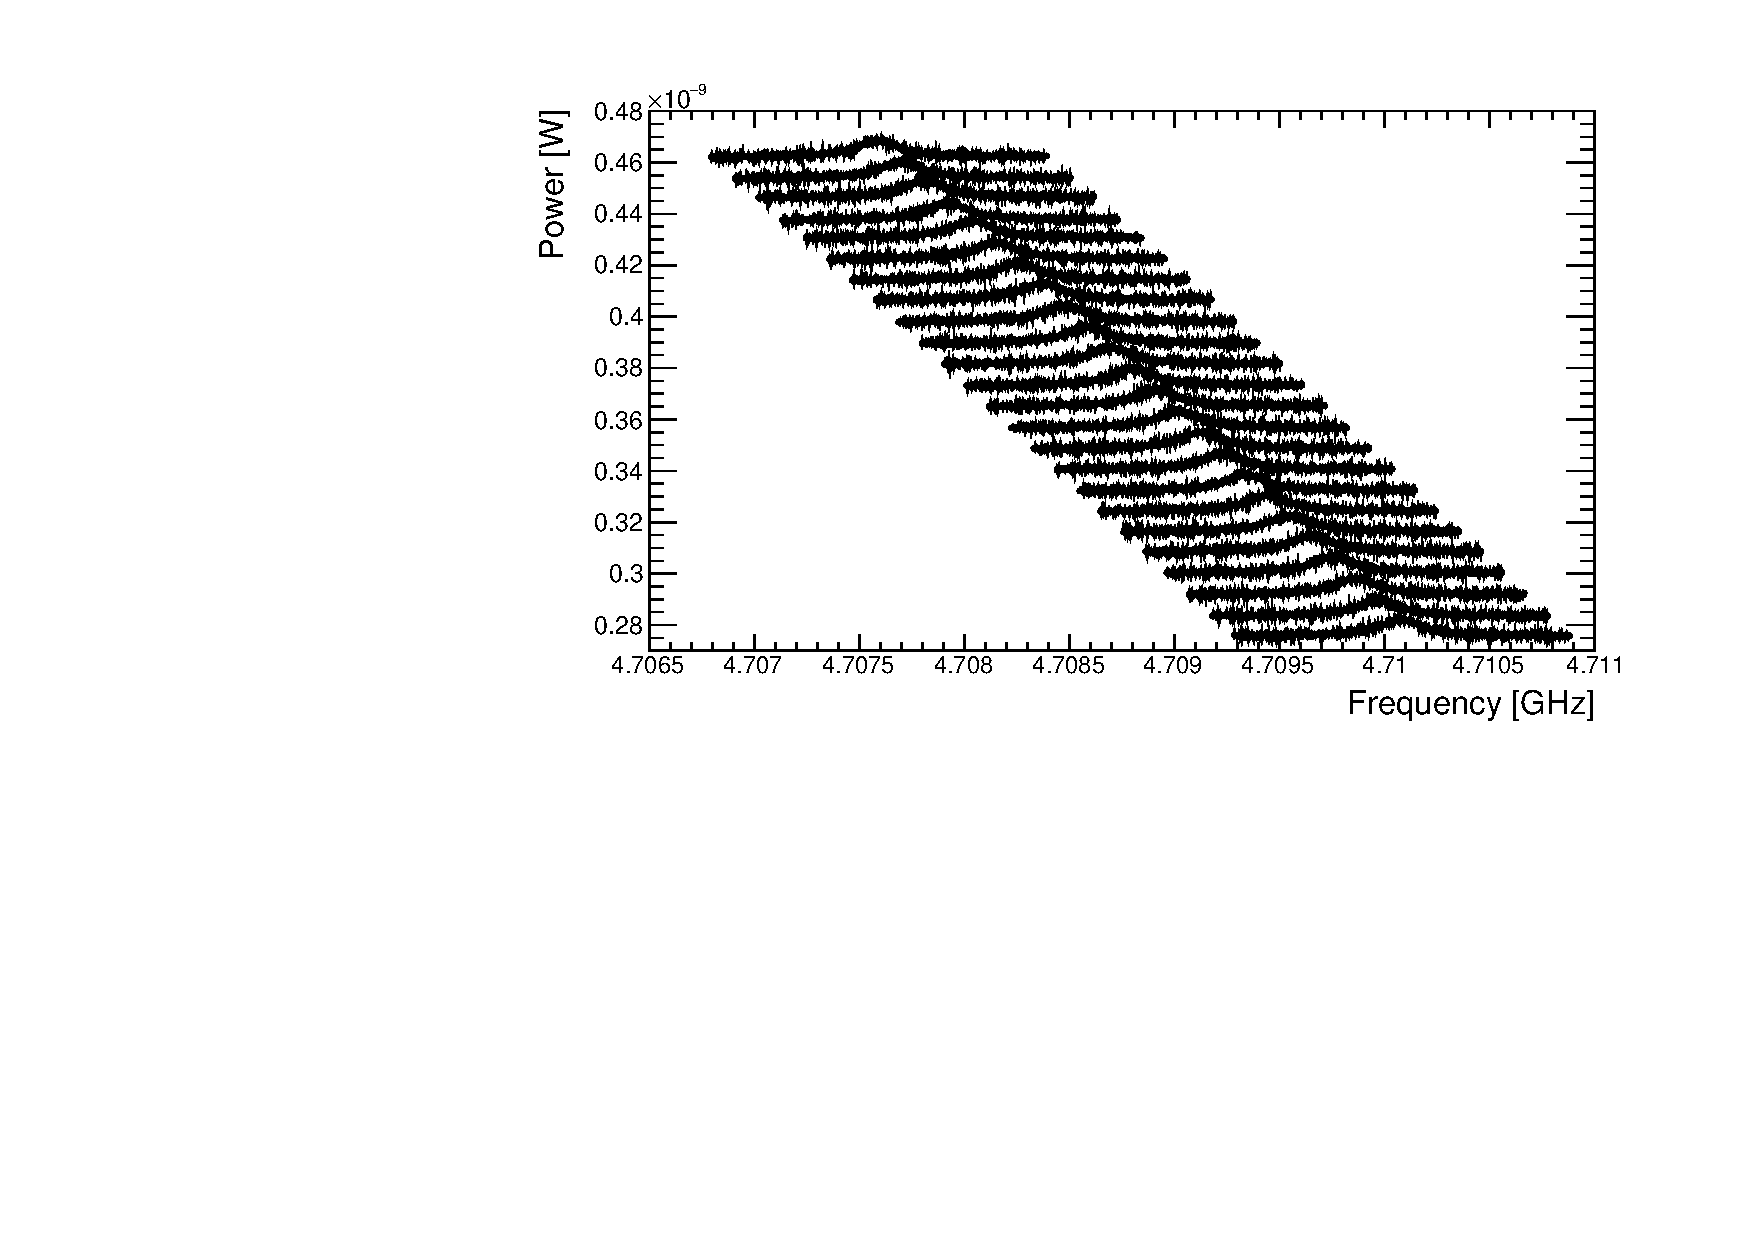
\includegraphics[width=0.48\textwidth]{figures/RawSpectra_Faxion_YAxis_Shifted.pdf}
    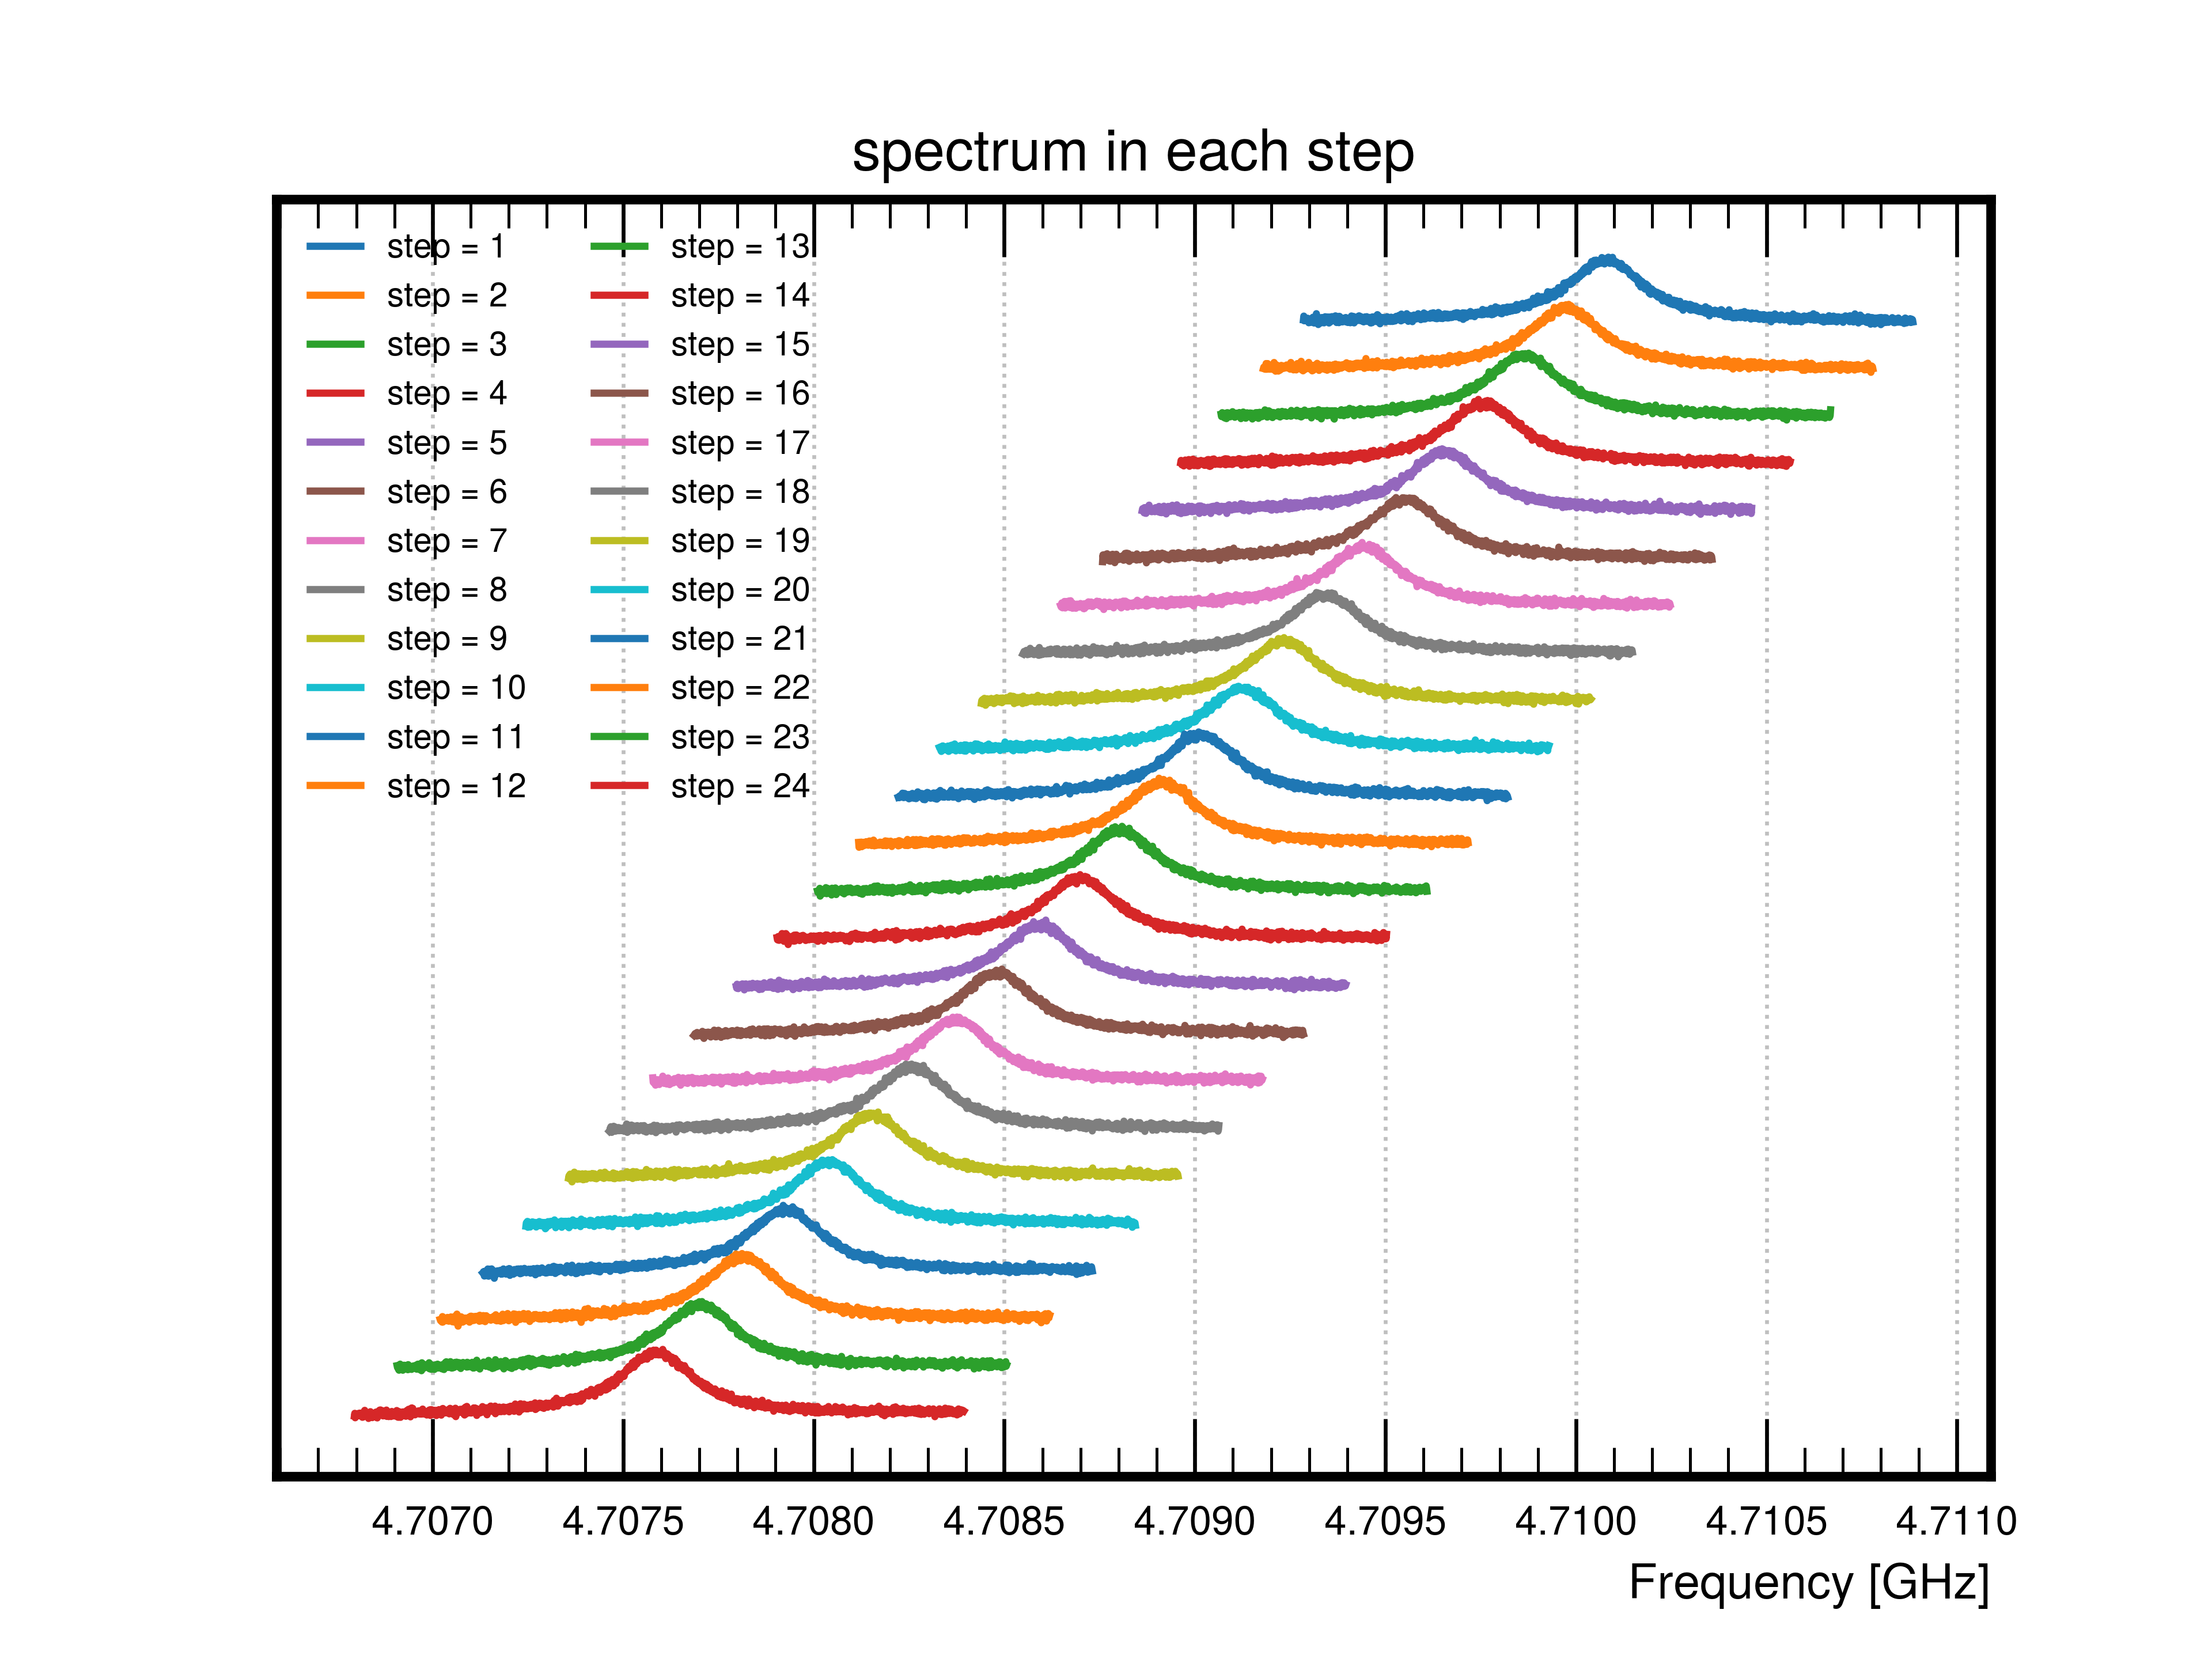
\includegraphics[width=8.6cm]{figures/faxion_rawpower_24steps.png}
 \caption{The raw output power spectra, before applying the 
 SG filter, from the 24 frequency steps of the synthetic axion 
data. In order to show the spectra clearly, the spectra are shifted 
with respect to each other with an arbitrary offset in the vertical scale.}                
\label{fig:faxionstep}                                                                                                            
\end{figure}                       

\begin{figure}[htbp]                                                                                                  
    \centering                                                                                                                       
    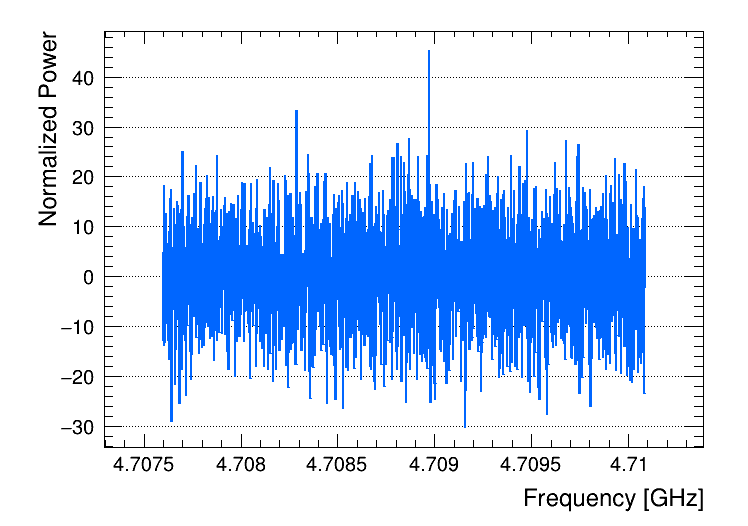
\includegraphics[width=8.6cm]{figures/Power_CombSpectrum_FaxionRun_AllSteps_Rescan_SG4_W201.png}
    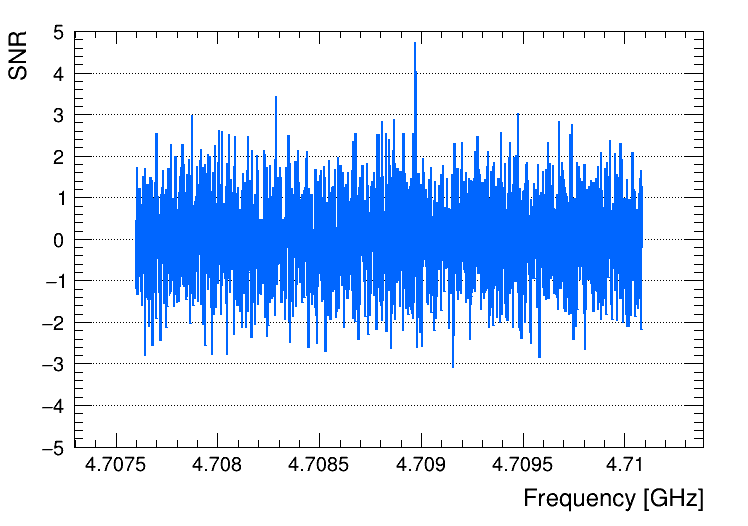
\includegraphics[width=8.6cm]{figures/SNR_CombSpectrum_FaxionRun_AllSteps_Rescan_SG4_W201.png}
    \caption{The RDP (upper) and the 
signal-to-noise ratio (lower) after combining the spectra 
of the synthetic axion data with overlapping frequencies from different scans.
 The procedure and the weights for combination are summarized in 
Sec.~\ref{sec:weighting_algorithm}.}                
\label{fig:faxioncombine}                                                                                                            
\end{figure}                       


\begin{figure}[htbp]                                                                                                  
    \centering                                                                                                                       
    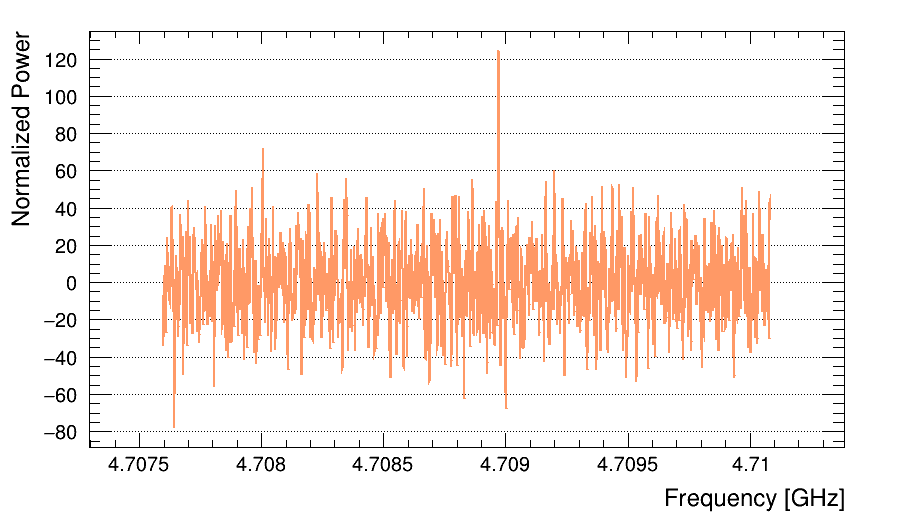
\includegraphics[width=8.6cm]{figures/Power_GrandSpectrum_FaxionRun_AllSteps_Rescan_Merged_5bin_SG4_W201_LqWeight.png}
    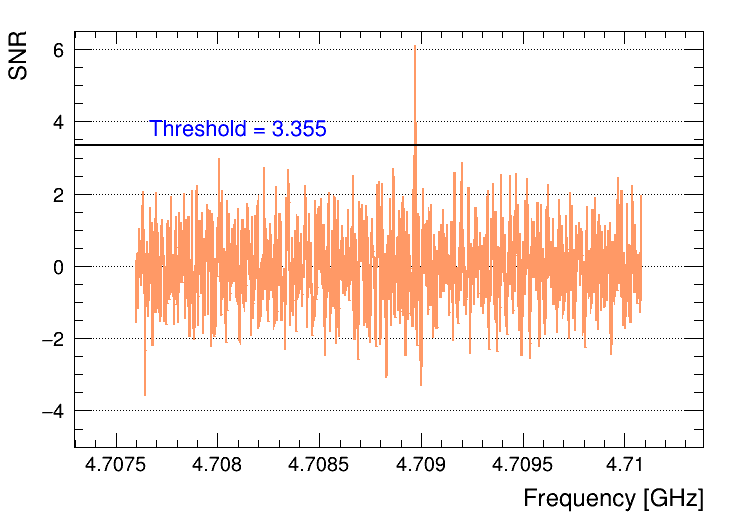
\includegraphics[width=8.6cm]{figures/SNR_GrandSpectrum_FaxionRun_AllSteps_Rescan_Merged_5bin_SG4_W201_LqWeight.png}
    \caption{The RDP (upper) and the signal-to-noise ratio (lower) after 
merging the RDP measured in five neighboring frequency bins of the 
synthetic axion data. 
The procedure and the weights for merging 
are summarized in Sec.~\ref{sec:merge}.}                
\label{fig:faxionmerge}    
\end{figure}                       

   
